\chapter{Methodology}\label{ch:style}

This chapter aims to outline the work undertaken throughout thesis A, B, and C, and the working code in thesis C.

This thesis aimed to develop a pipeline that is able to:
\begin{enumerate}
    \item Clean and label raw mmWave data for training.
    \item Process raw mmWave data into frame sequences.
    \item Data Splitting.
    \item Develop a generative model to reconstruct frame sequences.
    \item Threshold code to determine if a fall occurred. 
\end{enumerate}

Figure 3.1 gives a high-level overview of the project, generalised flow, and pipeline.

\begin{figure}[H]
    \centering
    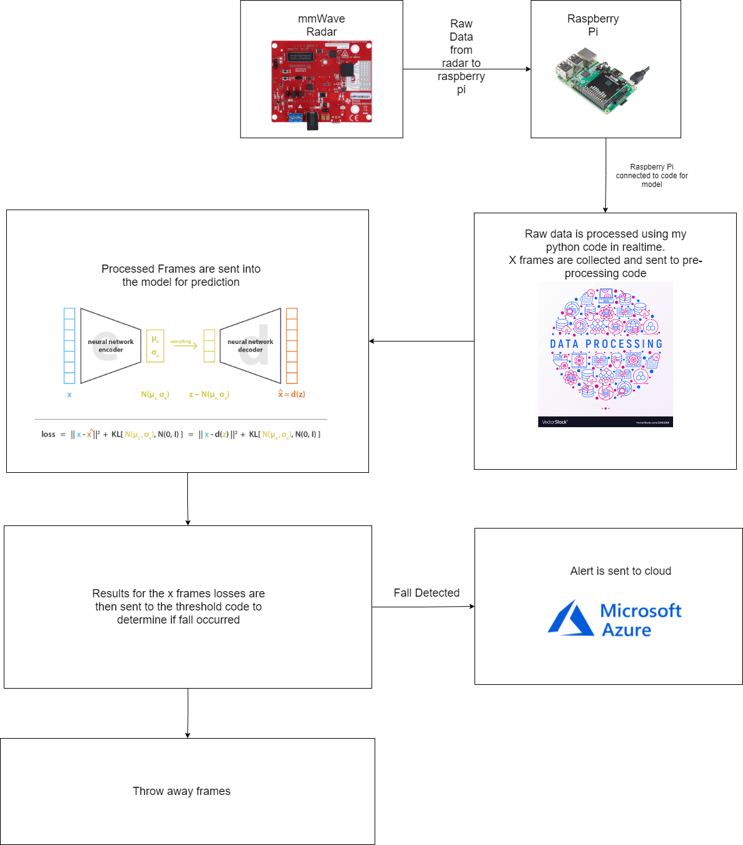
\includegraphics[width=425px,keepaspectratio=true]{tech.png}
    \caption{Generalised pipeline of thesis project.}
    \label{fig:my_label}
\end{figure}

\section{Data Cleaning and Structuring}
The aim of data cleaning was to create structured and labelled data out of the raw mmWave sensor output. This process also involved the removal of outliers and invalid data points obtained from the sensor. Participant data from the sensor arrives as one big point cloud dump containing information on the following:
\begin{itemize}
    \item Timestamp
    \item Frame Number
    \item xyz Coordinates
    \item Doppler
    \item SNR
    \item Range
    \item Azimuth
    \item Elevation
\end{itemize}

Figure 3.2 illustrates a sample subject folder containing all the point cloud information for all activities performed by the subject during that day. Inside of the points\_cloud.csv file we have the raw sensor data used for constructing frame sequences. Inside the track\_ids.csv file we have target tracking information associated with each point in the points\_cloud.csv file. Finally, the target\_list.csv file contains information about all targets that are found in the track\_ids.csv file.

\begin{figure}[H]
    \centering
    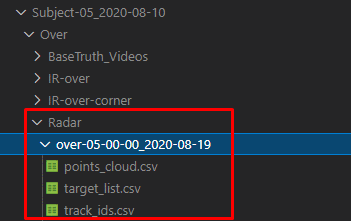
\includegraphics{raw_data.png}
    \caption{Participant data output file structure.}
    \label{fig:my_label}
\end{figure}

Figure 3.3 shows the content of the points\_cloud.csv file in Figure 3.1. As shown below, there is no structure to this data, and there is no way of determining which activity is which based on the data we have based on the data's current form. 

\begin{figure}[H]
    \centering
    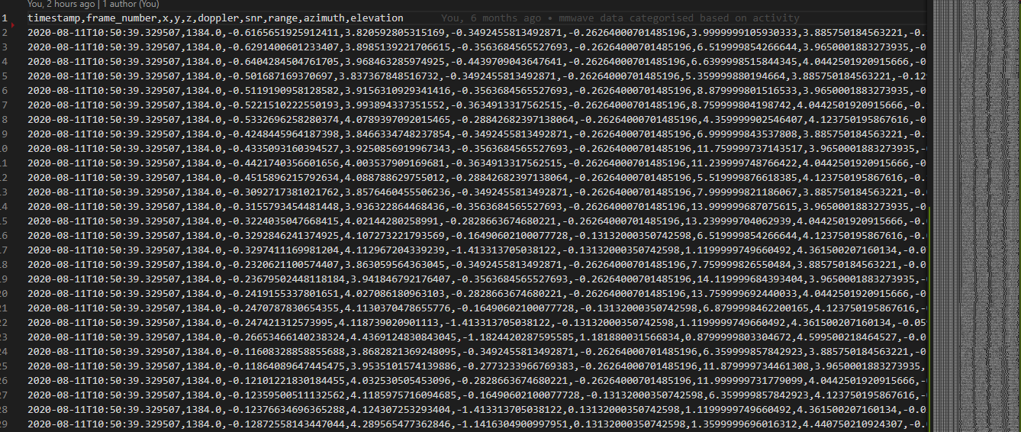
\includegraphics[width=425px,height=270px]{raw_dump.png}
    \caption{Contents of sample points\_cloud.csv file.}
    \label{fig:my_label}
\end{figure}

I resolved the issue of unstructured data by developing a flexible python script that is able to link the raw points\_cloud.csv file to the corresponding ground truth file that contains the duration of each activity. Using this information I can calculate how many frames are in each activity and the order in which they occur in. After synchronizing the clocks between the mmWave sensor and the ground truth video camera, I was able to go through the massive points\_cloud.csv file and determine which activity had occurred and the number of frames for said activity. I had created sub-samples that only contain the data for the activity. These sub-samples look identical to the original points\_cloud.csv in terms of structure. Figures 3.4 demonstrate the result of data cleaning, where the files are labelled based on which directory they are saved in. This powerful script allows for labelling the unstructured data based on activity. 

\begin{figure}[H]
    \centering
    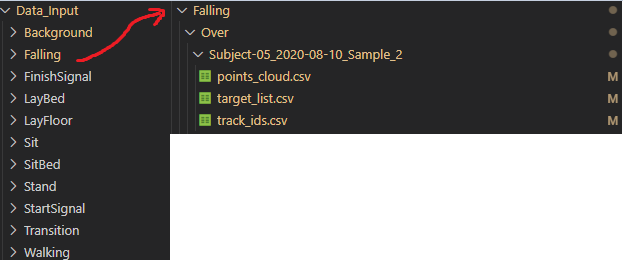
\includegraphics{result.png}
    \caption{Output sample of data cleaning script.}
    \label{fig:my_label}
\end{figure}

\section{Data Pre-Processing}
For any machine learning project, data pre-processing is the most important step, and correct execution is crucial to acquire meaningful results. The data pre-processing pipeline had the following steps in order to turn the raw mmWave data into frame sequences.
\begin{enumerate}
    \item Loading all raw data and categorising the data by activity.
    \item Generating frames from this data by grouping data points.
    \item Generating frame sequences by using a sliding window to move across the frame arrays.
    \item Oversampling each frame in the sequence to ensure all frames are of equal length.
    \item Saving and loading these frame sequences.
\end{enumerate}
\subsection{Loading Data}
Raw mmWave data is loaded into the program through the use of a map. The map enables the categorization of raw data loaded from points cloud.csv files. Each activity consists of a number of samples and is represented in the program as an array of sample data for map value. The map is of the following structure Map$<$Activity, [Sample]$>$. The script parses all activities, and for each sample in said activity, the points\_cloud.csv file is loaded and stored in the map as a numpy array under the corresponding activity.

\subsection{Generating Frames and Frame Sequencing}
To generate frames out of raw mmWave point data, we go through each sample one at a time and group together points that have the same timestamp using a map. The map is of the following structure  Map$<$Frame, [Point]$>$. Due to overlapping timestamps across samples, the sample name was also combined with the Frame key to generate a unique timestamp for each sample. 

Once frames were generated, the next step was to perform frame sequencing. First,  the map is flattened into an array. Next, each frame is scanned for invalid points and invalid data. With this array of frames, a sliding window is used with a customisable step size to move across the array and generate frame sequences for each sample. The size of each frame sequence is a customisable parameter set by the user. 

\subsection{Oversampling}
Ensuring all frames are of the same size is crucial for a machine learning model, as models only work with static input size. Due to the variable nature of point cloud data, all frames have a different number of points. In order to standardise input into the model, all frames are oversampled to the largest possible frame size. The largest frame size is computed during the frame generation as an optimisation step, constantly updating the maximum, rather than recomputing through a linear search. The oversampling technique used is based on a paper written by \textit{Jin et al.} [15] where the number of points in a frame are extended, whilst keeping the same distribution. 

\subsection{Saving and Loading}
Oversampling the frame sequence concludes the final step of the data pre-processing pipeline. Due to the tedious and complex nature of data pre-processing, checkpointing data that has already been pre-processed saves a tremendous amount of time when running the program. Every sample that had all its frame sequences oversampled is saved into a numpy file. When performing data pre-processing we ignore all samples that have been already saved.

To work with the saved data, a function is created to load all saved samples and store them in a map based on their activities. 

\section{Data Splitting}
To ensure that the model can be trained and tested correctly, appropriate data splitting must be performed. The most important aspect when it comes to splitting the dataset is to capture the split percentage across all activities. Initially, I was taking the percentage across the whole dataset from start to finish, resulting in certain splits missing activities. In order to counteract this issue, I had taken the percentage of samples across all activities by traversing the activity map. Figure 3.5 displays a visual representation of taking an 80\% split of the dataset. It can be noted that the correct splitting technique that was implemented captures all activities across any split.

\begin{figure}[H]
    \centering
    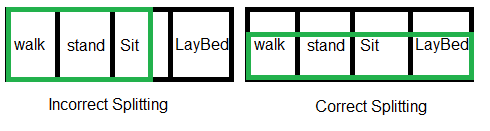
\includegraphics{split.png}
    \caption{Different possible data splitting techniques, right technique implemented.}
    \label{fig:my_label}
\end{figure}

Through the use of this data splitting technique, I was able to construct subsets of the original data in order to perform training, threshold calculation, and threshold evaluation. The following splits were performed:
\begin{itemize}
    \item Training the model: 80\% of non-fall samples
    \item Computing the threshold: 50\% of fall samples, 10\% of non fall-samples
    \item validating threshold and testing: 50\% of fall samples, 10\% of non fall-samples
\end{itemize}
Figure 3.6 gives a visual view of the data splitting that was performed.

\begin{figure}[H]
    \centering
    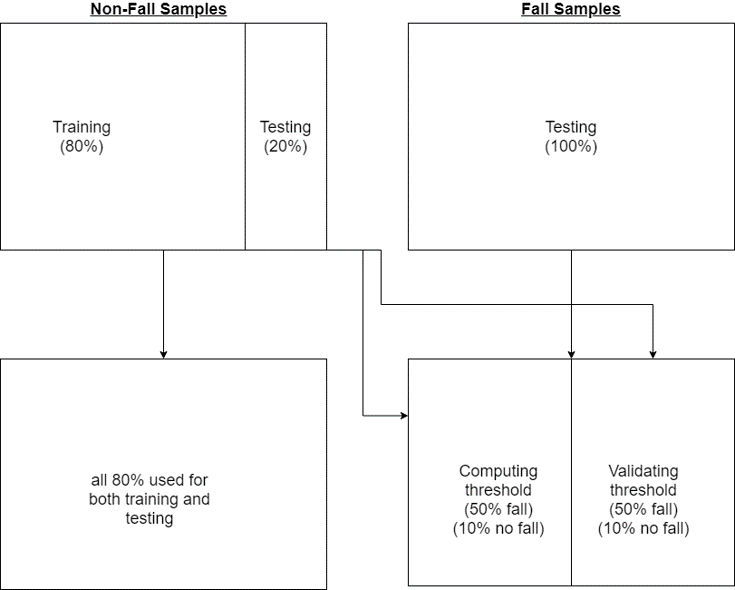
\includegraphics[width=330px, keepaspectratio=true]{splitting.png}
    \caption{Different possible data splitting techniques, right technique implemented}
    \label{fig:my_label}
\end{figure}

\section{Model Development}
The model developed for this paper was created using Tensorflow and Keras. A Variational Autoencoder (VAE) was constructed using a Recurrent Neural Network (RNN) as the bottleneck. This model was influenced from the paper written by \textit{Jin et al.} [15]. RNN models allow for effective information capture from data that relies on previous information. For this reason, an RNN was chosen over the traditional linear layer at the bottleneck. The input to the model is a series of frame sequences in the following format [x, window\_size, max\_frame\_size, 4]. X represents how many frame sequences are being passed into the model (x = 1 in real-time). Window size is a customisable hyper-parameter that determines how many frames are being reconstructed at once. Finally, the max frame size is the largest number of points in a single frame, all frames are oversampled to match this size. The output of the model is a combination of the input mean and input log variance which is used to compute the reconstruction loss of the network. The layers to the network developed are the following:
\begin{enumerate}[noitemsep, topsep=0px]
    \item Input: Input layer [?, 20, 288, 4]
    \item Encoding: Linear layer flatten inputs [?, 20, 288, 4] $\to$ [?, 20, 1152]
    \item Encoding: Dense encoding layer (shrink input) [?, 20, 1152] $\to$ [?, 20, 288]
    \item Encoding: Input mean dense layer [?, 20, 288] $\to$ [?, 20, 72] \\ Encoding: Input log variance layer [?, 20, 288] $\to$ [?, 20, 72]
    \item Encoding: Sampling layer [?, 20, 72] and [?, 20, 72] $\to$ [?, 20, 72]
    \item Bottleneck: Simple RNN layer [?, 20, 72] $\to$ [?, 72]
    \item Bottleneck: RepeatVector with 20 repeats [?, 72] $\to$ [?, 20, 72]
    \item Bottleneck: Simple RNN layer [?, 20, 72] $\to$ [?, 20, 72]
    \item Decoding: RNN output layer [?, 20, 72] $\to$ [?, 20, 72]
    \item Decoding: Dense decoding layer (expand input) [?, 20, 72] $\to$ [?, 20, 288]
    \item Decoding: reconstructed mean layer [?, 20, 288] $\to$ [?, 20, 4] \\ Decoding: reconstructed log variance [?, 20, 288] $\to$ [?, 20, 4]
    \item Decoding: combination layer (Concatenate) [?, 20, 4] and [?, 20, 4] $\to$ [?, 20, 8]
    \item Decoding: RepeatVector with 288 repeats [?, 20, 8] $\to$ [?, 20, 288, 8] 
    \item Output: Linear Layer [?, 20, 288, 8] $\to$ [?, 20, 288, 8]
\end{enumerate}

Figure 3.7 gives a visual representation of the VAE that was developed. 

\begin{figure}[H]
    \centering
    \includegraphics[width=375px, keepaspectratio=true]{model.png}
    \caption{Variational Autoencoder model with all layers involved}
    \label{fig:my_label}
\end{figure}

Using the output of this network, we are able to compute the reconstruction loss using the traditional VAE loss function. \textit{Rocca J.} [31] explains that VAEs are optimised to maximise the probability that "$x^{*} = x$" (probability our reconstructed output is the input) when we sample $z$ from the distribution $q^{*}_{x}(z)$ and then sampling $x^{*}$ from the distribution $p(x|z)$. In other words, we want to maximise the likelihood of the reconstructed input whilst staying close to the distribution of our input. To achieve this behaviour we can maximise the expected log-likelihood whilst minimising the KL divergence between our distributions. The following loss function was implemented in python.
\begin{center}$\mathbb{E}_{Q}[logP(x|z)] - KL(Q(Z)||P(Z)) $\end{center}

\section{Thresholding}
Given the output of the model is a single loss value representing reconstruction loss, and the binary nature of our classification problem, thresholding will allow us to distinguish between two output classes. Our model is trained to reconstruct ADL activities giving us overall a lower reconstruction loss on ADL data. When other activities are reconstructed through the model, there is a higher reconstruction loss as the model has not been trained on these types of activities. The key benefit to semi-supervised learning is that we don't need to train using fall data to predict falls, however, this requires a fine-tuned threshold to distinguish between abnormalities and regular activity data. This project aims to predict falls in a manner that maximises the true positive rate whilst minimising the false alarm rates. Rather than performing multi-variable optimisation on two separate values, we had used Youden's Index to create one value that is the true positive rate minus the false positive rate. The aim is then to maximise the Youdin's Index to determine an optimal threshold for distinguishing falls and ADL.

It is worth noting that thresholding creates a trade-off for overall model accuracy, a higher threshold will result in less accuracy on fall samples but a higher accuracy on ADL samples, and vice-versa. This makes the aim of our threshold to find an equilibrium between ADL and fall accuracy, whilst also allowing for the ability to adjust the threshold to suit specific performance requirements. 


\section{Technologies}
The language of choice for the entire project was python. All data pre-processing and algorithms are carried out in python due to the simplistic nature of python code. Data pre-processing is a complex task that required many algorithms involving linking multiple files together. If performance was a requirement, the code would have been performed in C++. To develop the model TensorFlow and Keras were the chosen machine learning framework. The team I had worked with had collaborated using bitbucket as well as a shared scratch on katana for a centralised dataset. Figure 3.8 gives a visual overview of the architecture and technology used throughout the project.

\begin{figure}[H]
    \centering
    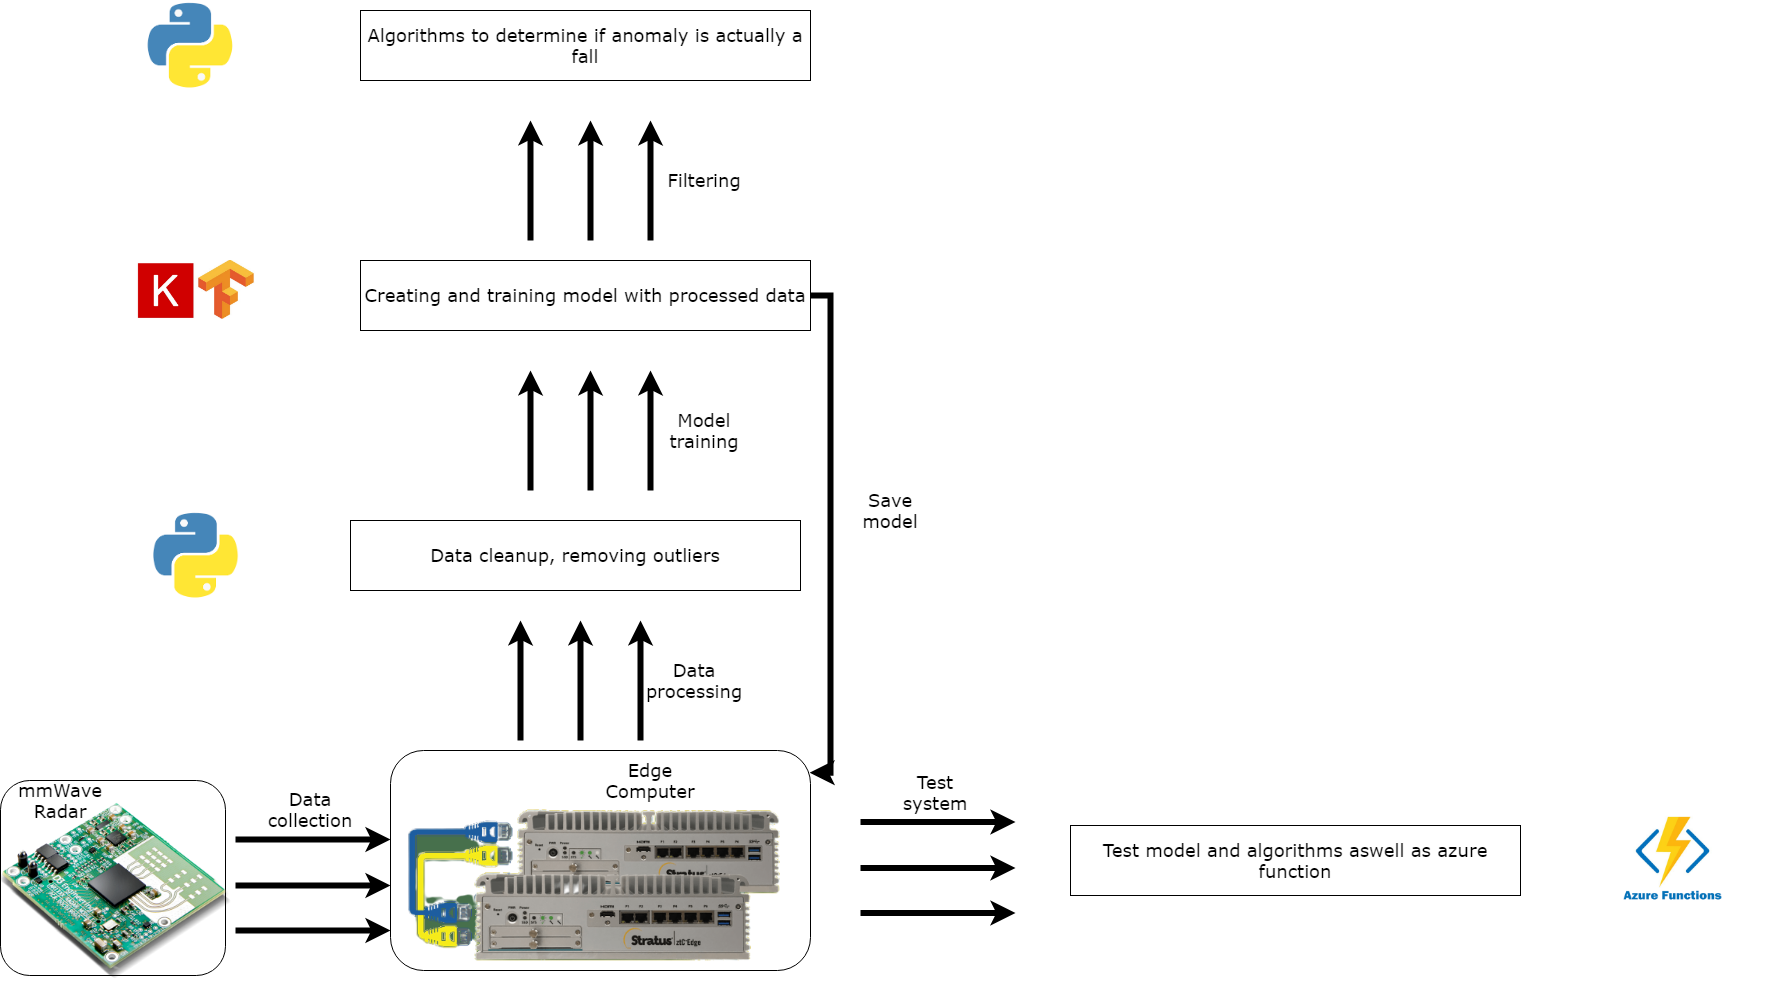
\includegraphics[width=500px, keepaspectratio=true]{archtrain.png}
    \caption{Architecture used for this project}
    \label{fig:my_label}
\end{figure}